\documentclass[12pt]{article}
\usepackage[utf8]{inputenc}
\usepackage[russian]{babel} 
\usepackage{graphicx}
\DeclareGraphicsExtensions{.pdf,.png,.jpg}
\pagestyle{empty}
 \usepackage[left=20mm, top=20mm, right=20mm, bottom=10mm, nohead, nofoot]{geometry}
 
    \begin{document}
    \section{Криптография простым языком: разбираем симметричное и асимметричное шифрование на примере сюжета Звездных войн (Updated)}
    
    
    Привет всем читателям Хабра! Не так давно решил разобраться с алгоритмами шифрования и принципами работы электронной подписи. Тема, я считаю, интересная и актуальная. В процессе изучения попробовал несколько библиотек, однако самой удобной с моей точки зрения является библиотека PyCrypto. У неё прекрасная документация, сопровождаемая примерами.
    
    \begin{center}
    
\includegraphics[width=1\linewidth]{pictures/img1.jpg}
    \end{center}
    
    
    \textbf{После прочтения материала вы усвоите следующие моменты:}
    
   \begin{enumerate} 
    \item Что такое шифрование;
    \item Чем отличается симметричное шифрование от асимметричного;
    \item В каком случае эффективнее применять симметричное, а в каких асимметричное шифрование;
    \item Что такое хеш данных и для чего он используется в шифровании;
    
\end{enumerate}
    
    
    Актуальность рассматриваемой темы постоянно растет. Применение криптографии уже давно не ограничивается шифрованием информации. Алгоритмы шифрования в том или ином виде ежедневно используется нами при посещении сайтов через протокол HTTPS, во время совершения покупок банковской картой, при общении в мессенджерах. Последние несколько лет широкое внимание привлекают блокчейн технологии, основой которых также является криптография.
    
    \vspace{0.5cm}
    Целью данной статьи является познакомить читателя с основными алгоритмами шифрования. При написании статьи, я постарался как можно большее внимание уделить вопросу практического применения. Для программирования использовался язык Python 3.6. При написании кода старался делить его на отдельные части и комментировать все ключевые моменты.
    \vspace{0.5cm}
    
    В данной статье я не разбирал цифровую подпись, однако после понимания асимметричного шифрования смысл этой технологии станет понятен.
    
    \subsection{Сюжет}
    Давайте мысленно перенесемся во вселенную Звездных войн до событий Эпизода 6, когда силам сопротивления становится известно о начале строительства новой Звезды смерти. Командование планирует внедрить разведывательную группу под видом строителей. Операция очень опасна, связь со штабом будет затруднена. В случае экстренной стиуации каждый член группы может отправлять и получать сообщения из штаба на незащищенной частоте.
    \vspace{0.5cm}
    Целью разведгруппы являются любые данные, которые могут пролить свет на конфигурацию, вооружение и назначение будущей станции. Для хранения данных планируется разработать специальное оборудование и ПО.
    
    \vspace{0.5cm}
    
    \textbf{Штаб утвердил два варианта этой операции:}
    
    \vspace{0.5cm}
   
    План А — возвращение агентов с данными повстанческим силам;
    \\
    План Б — дистанционная передача планов с самой Звезды смерти, используя оборудование станции.
    \\
    Передача информации при этом будет быстрой, но после передачи агент вероятнее всего будет вычислен и пойман.
    
    \vspace{0.5cm}
    
    Вы являетесь программистом в команде, которая отвечает за разработку ПО.
   
   \vspace{0.5cm}
    
   \textbf{ При планировании операции рассматриваются несколько возможных негативных сценариев:}
    
    \begin{itemize}
    	
    	\item Противник перехватит сигнал, поймет по его содержимому о планировании атаки и уведет объект ближе к лояльным Империи силам. В этом случае потери среди сопротивления будут выше;
    	
    	
    	\item Один из шпионов будет пойман и на допросе раскроет план операции, что может привести к компрометации ключей шифрования (про них будет сказано ниже);
    	
    	\item Шпион с загружеными данными может быть перехвачен имперскими силами, которые внесут изменения в содержимое, дезинформируя сопротивление о слабых местах станции. В этом случае, при атаке флот повстанцев будет направлен в ложном направлении и постепенно уничтожен;
    	
    \end{itemize}

	\textbf{Из этих сценариев смормулированы задачи:}
	
	\begin{enumerate}
		
		\item Содержимое должно быть надежно зашифровано и защищено от изменений;
		
		\item В случае утери ключей шифрования или их компрометации, должна быть возможность получения новых ключей шифрования дистанционно на частоте, которая может прослушиваться противником.
		
	\end{enumerate}

\subsection{Шифрование информации}
		Давайте решим проблему шифрования информации:
		
		\vspace{0.5cm}
		
		Для шифрования и дешифрования информации используется ключ шифрования. Именно ключ делает шифрование обратимым. Каждый агент будет снабжен ключом шифрования. После загрузки данных агент произведет их шифрацию и отправку в штаб сопротивления.
		
		\vspace{0.5cm}
		
		Метод, при котором шифрование и дешифрация сообщения производится при помощи одного ключа называется симметричное шифрование.
		
		 \begin{center}
			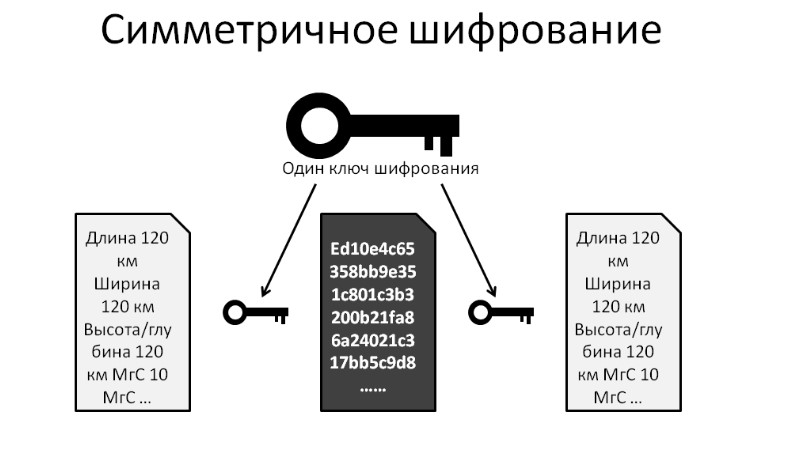
\includegraphics[width=1\linewidth]{pictures/img2.jpg}
		\end{center}
	
	\vspace{0.5cm}
	
	Слабым местом симметричного шифрования является ключ шифрования, точнее его доставка до адресата. Если во время доставки ключ будет скомпрометирован, стороннее лицо легко раскодирует сообщение. Сильной стороной симметричного шифрования является его скорость, что дает возможность кодировать большие объемы данных.
	
	\vspace{0.5cm}
	
	Асимметричное шифрование для кодирования данных использует два связанных друг с другом ключа: открытый и закрытый.
	
	\begin{center}
		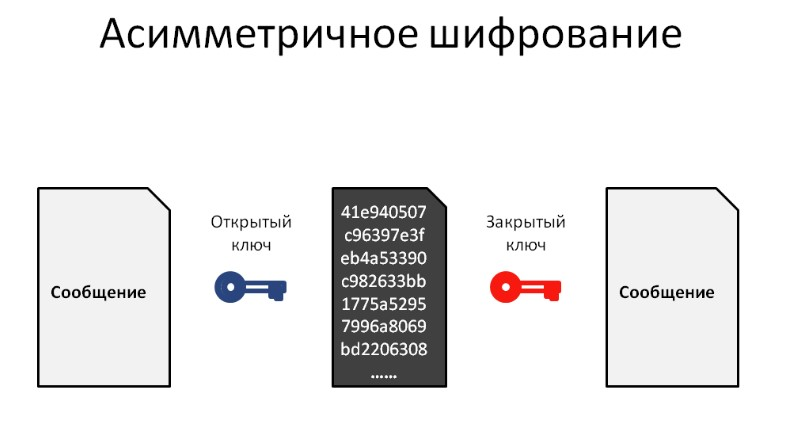
\includegraphics[width=1\linewidth]{pictures/img3.jpg}
	\end{center}
	
	\textbf{Механизм действия такой:}
	
	\begin{enumerate}
	\item адресат отправляет ОТКРЫТЫЙ ключ отправителю;
	\item отправитель кодирует сообщение при помощи полученного открытого ключа. При этом, раскодировать сообщение можно теперь только закрытым ключом;
	\item при получении зашифрованного сообщения адресат раскодирует его ЗАКРЫТЫМ ключом (который был сгенерирован в паре с открытым).
	
	\end{enumerate}
	\vspace{0.5cm}
	
	Для начала разработаем функционал для симметричного шифрования по названием Advanced Encryption Standard (AES). Он является одним из самых распространённых алгоритмов симметричного шифрования.
	
	\begin{center}
		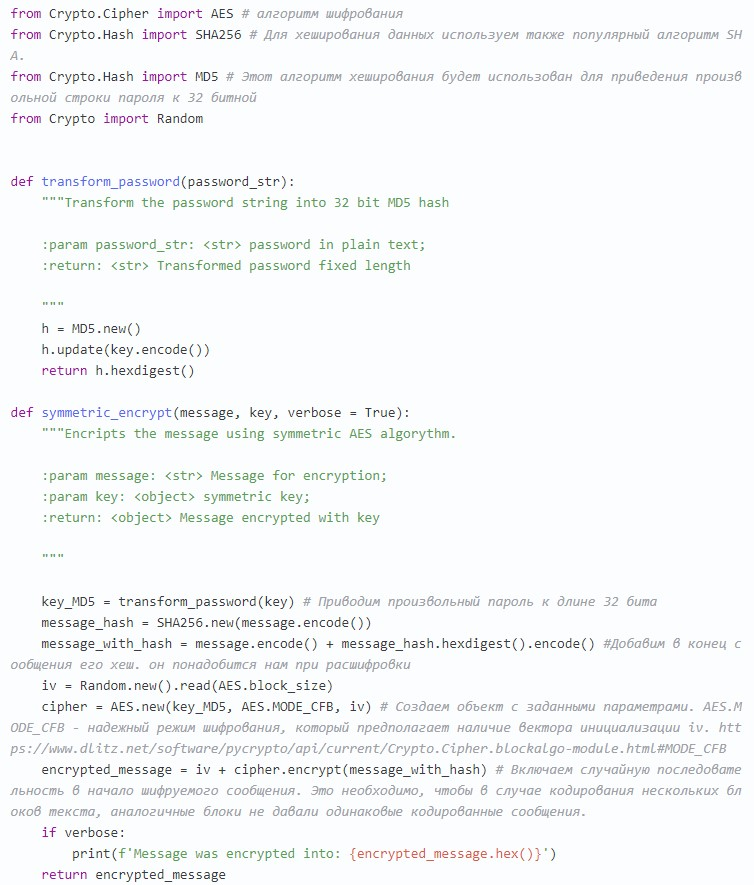
\includegraphics[width=1\linewidth]{pictures/code1.jpg}
	\end{center}

\begin{center}
	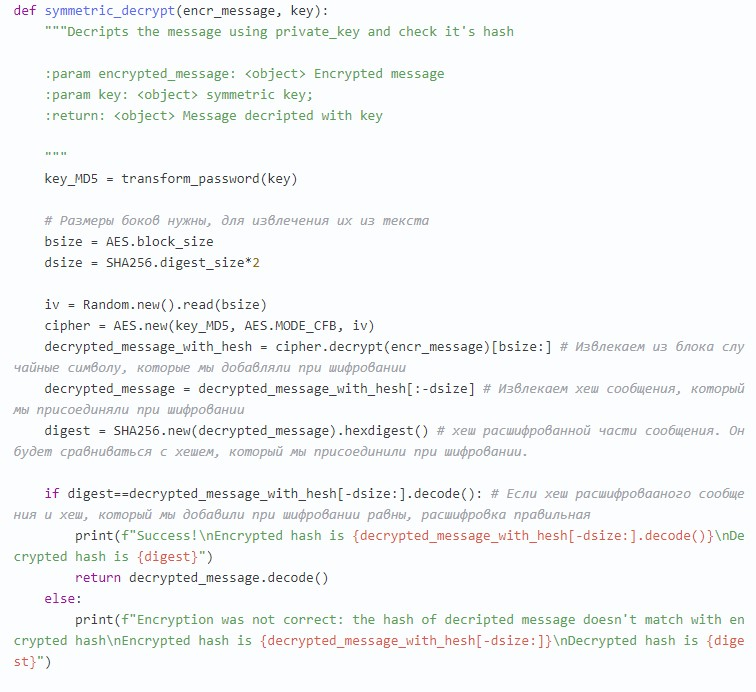
\includegraphics[width=1\linewidth]{pictures/code2.jpg}
\end{center}
\vspace{10cm}
	Проверим работоспособность кода на примере
	
	\begin{center}
		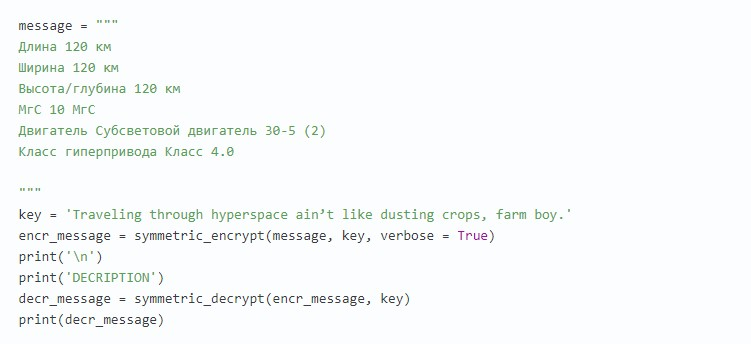
\includegraphics[width=1\linewidth]{pictures/code3.jpg}
	\end{center}
	
	\begin{center}
		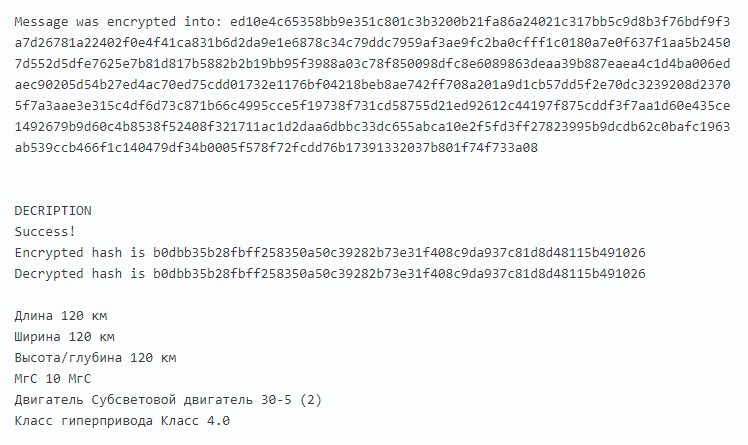
\includegraphics[width=1\linewidth]{pictures/code4.jpg}
	\end{center}

	Как видим, мы успешно зашифровали сообщение при помощи открытого ключа.
	Запустите код несколько раз. Вы увидите, что каждый раз зашифрованная часть меняется. Это происходит потому что при шифровании мы применили режим Cipher FeedBack (AES.MODECFB), при котором блоки открытого текста смешиваются с блоками шифротекста. iv — вектор инициализации (подробнее про режим читайте здесь). При расшифровке сообщения мы видим, что хеш расшифрованного сообщения совпадает с хешем, который мы добавляли при шифровании. Это значит, что дешифрация прошла корректно.
	
	\vspace{1cm}
	
	\subsection{Что такое хэш ?}
	
	Хеш документа — это просто строка из символов, которая уникальна для какого-либо набора данных. При любом изменении данных хеш очень сильно меняется. Другими словами, хеш — это своеобразный «отпечаток пальца» для какого-либо набора данных.
	
	\begin{center}
		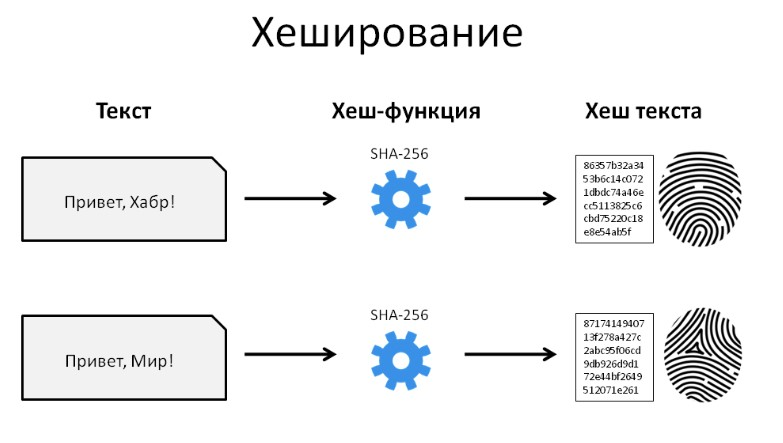
\includegraphics[width=1\linewidth]{pictures/img4.jpg}
	\end{center}

	Но что делать, если ключи шифрования будут по каким-то причинам скомпрометированы? Тогда расшифровать информацию может кто угодно.
	
	\vspace{0.5cm}
	
	В этом случае нам нужно как-то сменить ключи шифрования дистанционно по частоте, которая может прослушиваться противником. Будем считать, что ее уже слушают. Так каким же образом нам это сделать? Тут на помощь приходит другой метод под названием асимметричное шифрование (или криптографическая система с открытым ключом). В отличие от симметричного шифрования, при ней используется два ключа: открытый и закрытый. Сообщение шифруется открытым ключом, после этого расшифровать его можно только закрытым ключом. Открытый ключ при расшифровке будет бесполезен. Однако есть важный момент: закрытый ключ непременно должен быть из сгенерированной пары с открытым. Наличие открытого ключа одно из нескольких важных и интересных свойство асимметричного шифрования. То есть, мы можем передавать открытый ключ любым каналом и не бояться, что он будет применен для расшифровки сообщения.
	
	\vspace{0.5cm}
	
	Вместе с тем, применительно к нашей задаче есть один ньюанс — асимметричное шифрование подходит для небольших данных, например коротких сообщений. Мы можем только гадать об объеме данных, полученных разведкой. Мы, конечно, можем разбить все полученные данные на небольшие фрагменты и закодировать каждый из них закрытым ключом, но есть более оптимальный вариант решения.
	
	\textbf{Реение}
	
	Пользователь Akelawolf справедливо заметил, сгенерировать и отправить открытый ключ может кто угодно. Я внес некоторые коррективы в план.
	
	\vspace{0.5cm}
	
	Будет правильно, если до отправки агентов штаб сгенерирует несколько пар ключей и назначит каждому агенту закрытый ключ. Лучше сгенерировать именно несколько пар, чтобы у каждого агента был индивидуальный ключ. Это необходимо, чтобы точно персонифицировать владельца ключа.
	\\
	Тогда в случае компрометации ключей центр создаст новый СИММЕТРИЧНЫЙ ключ, закодирует его каждому агенту открытыми ключами и отправит по открытому каналу.
	
	\begin{center}
		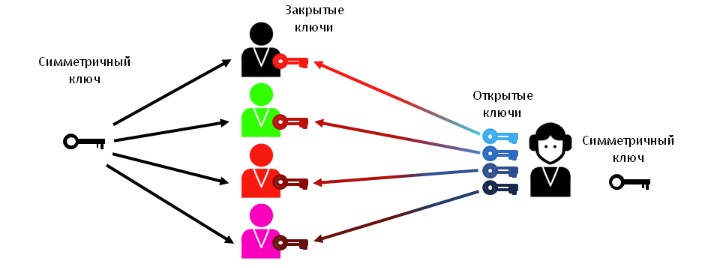
\includegraphics[width=1\linewidth]{pictures/img5.jpg}
	\end{center}

\begin{center}
	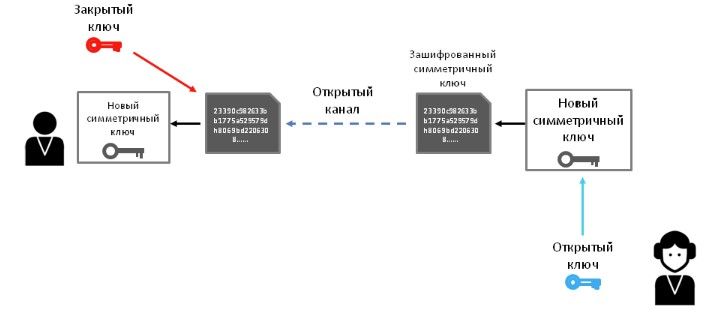
\includegraphics[width=1\linewidth]{pictures/img6.jpg}
\end{center}

	Старое решение
	
	\vspace{1cm}
	
	\begin{enumerate}
		\item Агент сгенерирует пару ключей (открытый и закрытый) на месте, затем отправит открытый ключ повстанческим силам;
		\item В штабе сопротивления создадут новый ключ для СИММЕТРИЧНОГО шифрования;
		\item Симметричный ключ закодируют при помощи открытого ключа, который прислал агент;
		\item Зашифрованный симметричный ключ отправят агенту, который раскодирует его с помощью закрытого ключа.
	\end{enumerate}
	
	Обратите внимание на нашу передачу по открытому каналу:
	
	\begin{enumerate}
		\item Агент отправляет ОТКРЫТЫЙ ключ из пары, ЗАКРЫТЫЙ ключ находится у него;
		
		\item Штаб сопротивления отправляет ключ симметричного шифрования, зашифрованный присланным агентом открытым ключом.
	\end{enumerate}

	\vspace{1cm}
	
	Ни первое ни второе сообщение не представляют какой-либо ценности при перехвате.
	
	\vspace{1cm}
	
	Напишем код:
	
		\begin{center}
		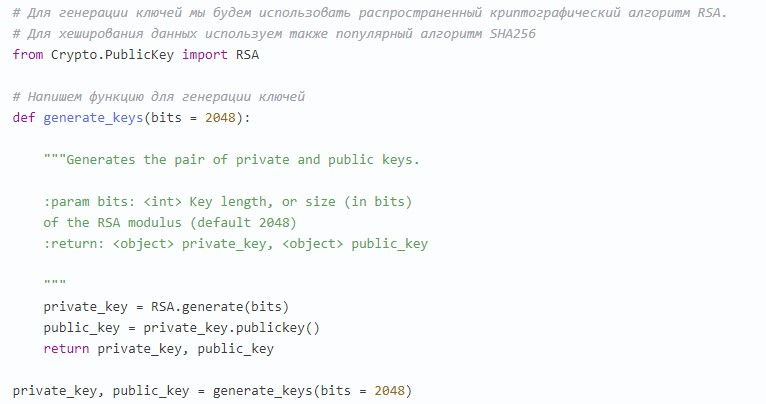
\includegraphics[width=1\linewidth]{pictures/code5.jpg}
	\end{center}

	Давайте посмотрим как выглядят ключи:
	
		\begin{center}
		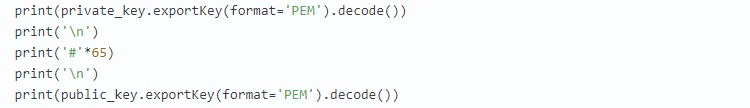
\includegraphics[width=1\linewidth]{pictures/code6.jpg}
	\end{center}

	\begin{center}
		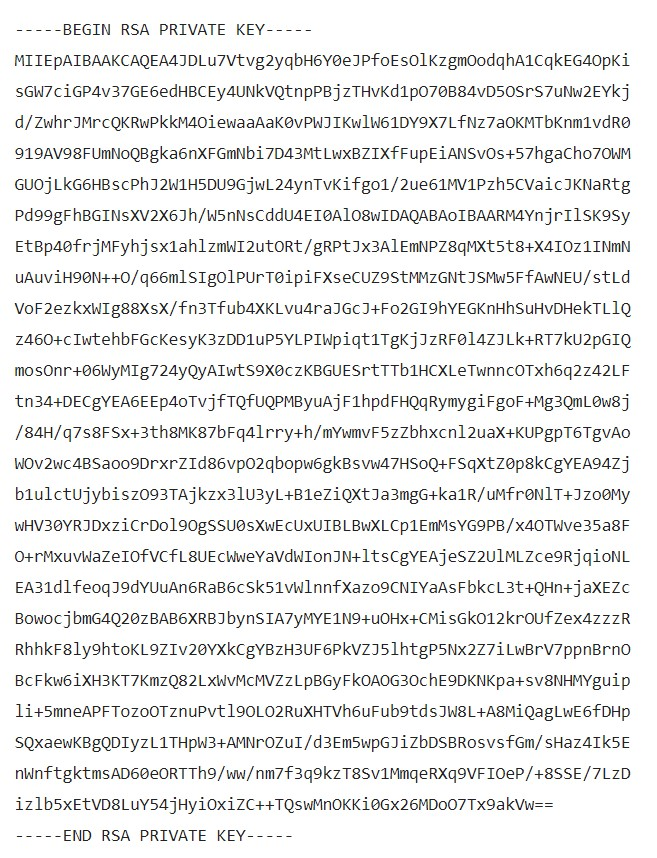
\includegraphics[width=1\linewidth]{pictures/key1.jpg}
	\end{center}

\begin{center}
	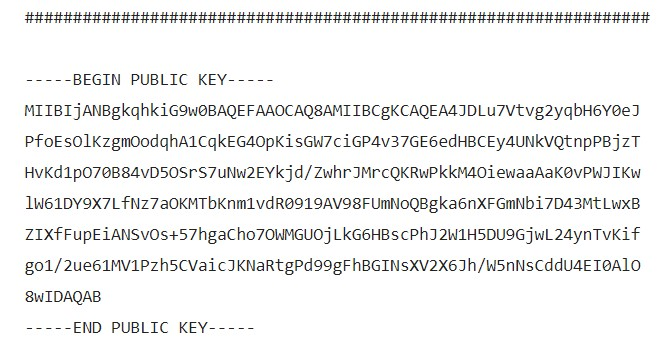
\includegraphics[width=1\linewidth]{pictures/key2.jpg}
\end{center}

	Как видите, ключи асимметричного шифрования представляют из себя длинные математически сгенерированные последовательности символов.
	
	\vspace{1cm}
	
	Итак, мы сгенерировали ключи. Теперь давайте напишем функцию для кодирования данных:
	
	\begin{center}
		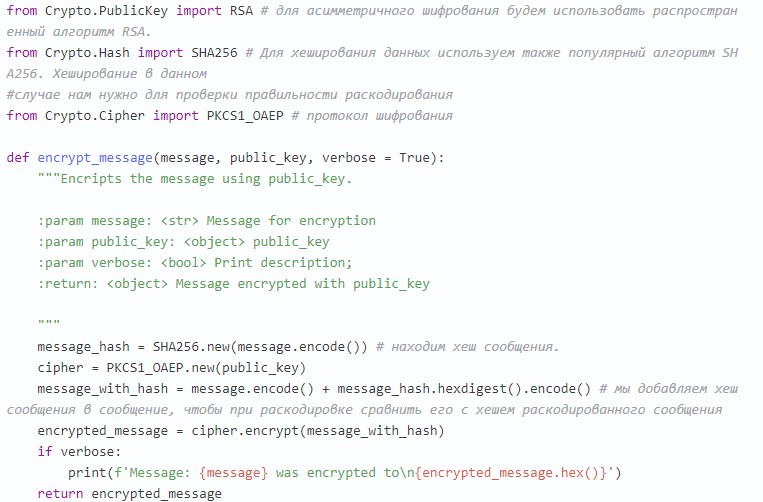
\includegraphics[width=1\linewidth]{pictures/code7.jpg}
	\end{center}

\begin{center}
	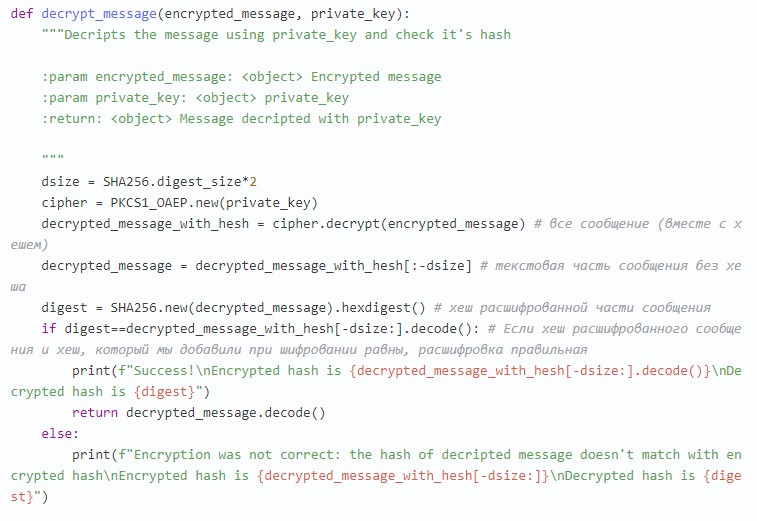
\includegraphics[width=1\linewidth]{pictures/code8.jpg}
\end{center}

	\textbf{Схема работы по шагам}
	\begin{enumerate}
		\item Агент генерирует пару ключей:
				\begin{center}
				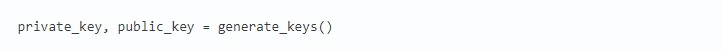
\includegraphics[width=1\linewidth]{pictures/code9.jpg}
				\end{center}
		\item Отправляет в штаб ОТКРЫТЫЙ ключ;
		
		\item В штабе с помощью открытого ключа кодируют ключ для симметричного шифрования:
				\begin{center}
					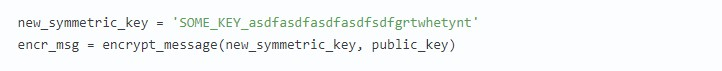
\includegraphics[width=1\linewidth]{pictures/code10.jpg}
				\end{center}
			Вывод	
			\vspace{1cm}
			Message: SOMEKEYasdfasdfasdfasdfsdfgrtwhetynt was encrypted to
			41e940507c96397e3feb4a53390c982633bb1775a52957996a8069bd22063086a0e831bf775a17909276aba0d0478ee6
			
			\item Эту длинную последовательность отправляют обратно агенту;
			\item Агент дешифрует полученное сообщение при помощи закрытого ключа:
				\begin{center}
					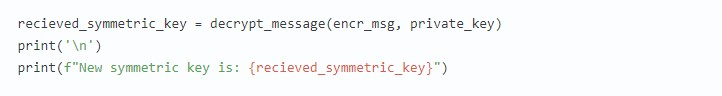
\includegraphics[width=1\linewidth]{pictures/code11.jpg}
				\end{center}
			
			Вывод
			
				\begin{center}
					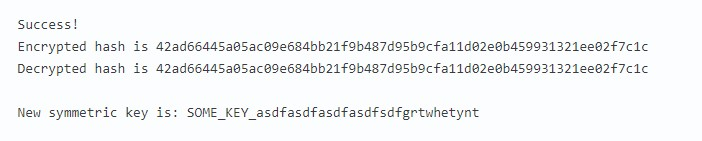
\includegraphics[width=1\linewidth]{pictures/code12.jpg}
				\end{center}
			
		\item Затем с помощью нового симметричного ключа агент шифрует полученные данные:
		
				\begin{center}
					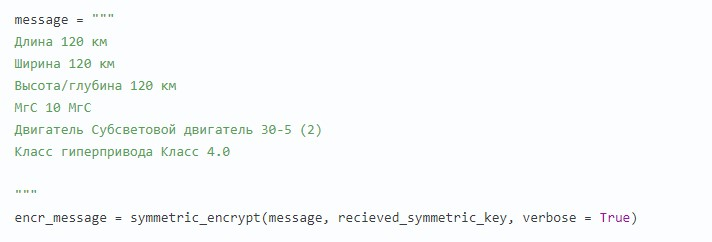
\includegraphics[width=1\linewidth]{pictures/code13.jpg}
				\end{center}
			Вывод
				
				\begin{center}
					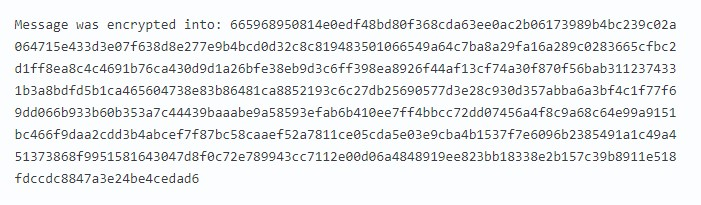
\includegraphics[width=1\linewidth]{pictures/code14.jpg}
				\end{center}
		\item В штабе производят дешифровку:
		
				\begin{center}
					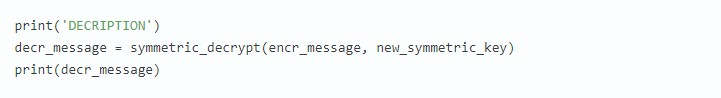
\includegraphics[width=1\linewidth]{pictures/code15.jpg}
				\end{center}
			Вывод
				
				\begin{center}
					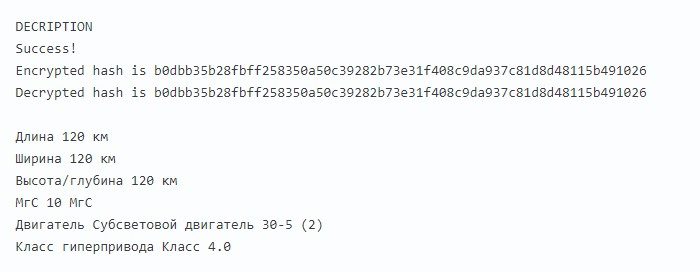
\includegraphics[width=1\linewidth]{pictures/code16.jpg}
				\end{center}
			
			\textbf{Вуаля}
			\vspace{1cm}
			
			На данном абстрактном примере мы увидели работу распространенных алгоритмов шифрования. Симметричное и асимметричное шифрование, а также хеширование применяются в работе веба, электронной подписи, блокчейне и криптовалютах. Надеюсь, материал был полезен для понимания работы этих технологий.
			
			\vspace{1cm}
			\textbf{Послесловие}
			\vspace{0.5cm}
			
			В итоге, разведке повстанцев удалось добыть точные сведения об уязвимости станции и пути до нее, присутствии Императора для осмотра, наличии энергощита и его источника на Эндоре. Империя вычислила шпионов, дезинформировала их о боеспособности станции. Станция также была отведена к спутнику Эндора, откуда была защищена щитом.
			
	\end{enumerate}
    \end{document}